\documentclass{standalone}
%outline around text
\usepackage[outline]{contour}
\contourlength{1.3pt}

%tikz
\usepackage{tikz}
\usetikzlibrary{knots, cd, calc}

\begin{document}
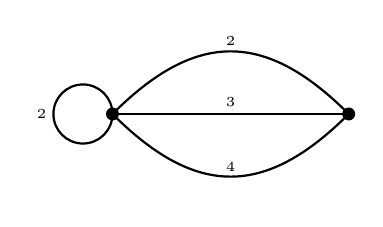
\begin{tikzpicture}[scale = 0.75]
\draw[thick] (0, 0) -- (4, 0);
\draw[thick] (0, 0) .. controls +(45:2) and +(315:-2) .. (4, 0);
\draw[thick] (0, 0) .. controls +(315:2) and +(45:-2) .. (4, 0);
\draw[thick] (-0.5, 0) circle (0.5);

\draw[fill = black] (0, 0) circle (0.1);
\draw[fill = black] (4, 0) circle (0.1);

\node at (2, 1.23) {\tiny{$2$}};
\node at (2, 0.2) {\tiny{$3$}};
\node at (2, -0.9) {\tiny{$4$}};
\node at (-1.2, 0) {\tiny{$2$}};
\end{tikzpicture}
\end{document}

